\documentclass{standalone}

\usepackage{tkz-fct}
\usepackage{tkz-euclide}
\usepackage{color}
\renewcommand*\familydefault{\sfdefault}
\usepackage{sansmath}
\sansmath
\definecolor{gray75}{gray}{0.75}
\begin{document}
 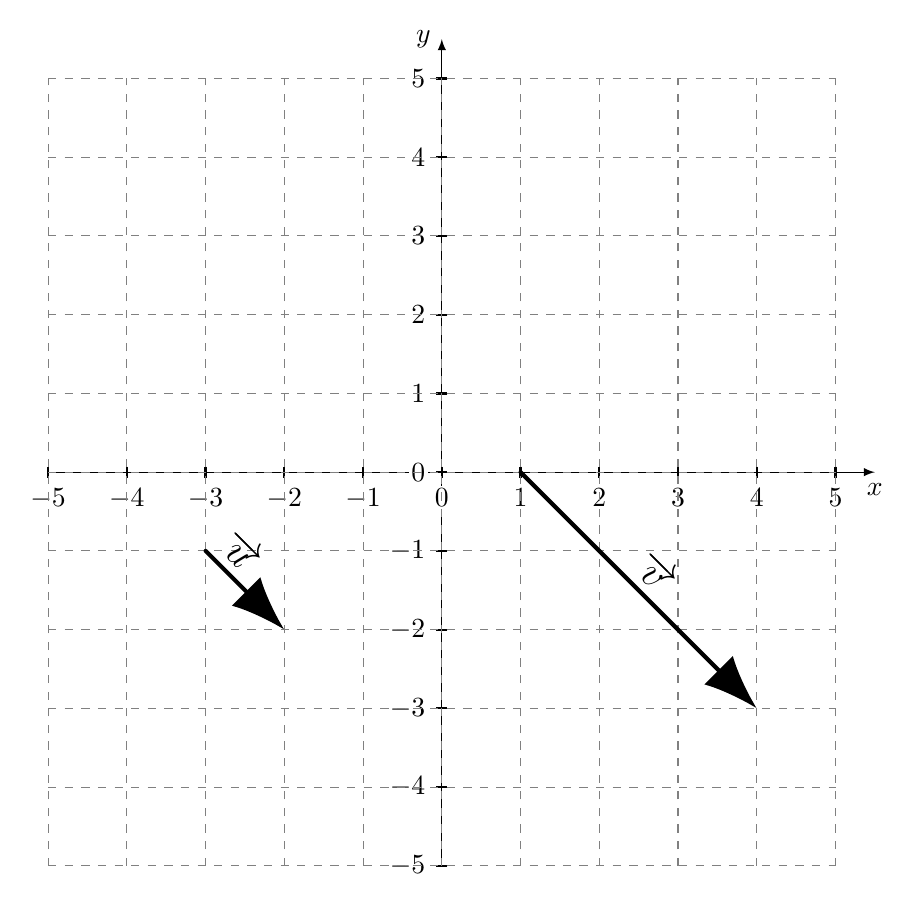
\begin{tikzpicture}
   \tkzInit[xmax=5,ymax=5,xmin=-5,ymin=-5]
   \tkzDrawX
   \tkzDrawY
   \tkzLabelX
   \tkzLabelY
   \begin{scope}[dashed]
     \tkzGrid
   \end{scope}
   \tikzset{vector style/.style={>={Latex[scale=2]},->}}
   \tkzDefPoints{-3/-1/A, -2/-2/B, 1/0/C, 4/-3/D, 7/1/E, 11/8/F, 10/0/G, 12/3.5/H}
   \tkzDrawSegment[line width=1.5pt,vector style](C,D)
   \tkzDrawSegment[line width=1.5pt,vector style](A,B)
   \tkzLabelSegment[above, sloped](C,D){\Large $\overrightarrow{v}$}
   \tkzLabelSegment[above left, sloped](A,B){\Large $\overrightarrow{u}$}

\end{tikzpicture}
\end{document}
